\documentclass[10pt,a4paper]{beamer}
\usetheme{Szeged}
\usecolortheme{beaver}
%\usefonttheme{serif}

\usepackage[utf8]{inputenc}
\usepackage{amsmath}
\usepackage{amsfonts}
\usepackage{amssymb}
\usepackage{inputenc}
\usepackage[lined,boxed,ruled,commentsnumbered]{algorithm2e}
\usepackage{pgfbaseimage}
\usepackage{subfigure}


\title % (optional, only for long titles)
{Análise de \textit{Timing} Estática e a Avaliação do Impacto do Atraso das Interconexões em Circuitos Digitais}
\author % (optional, for multiple authors)
{Chrystian de Sousa Guth}
\institute[UFSC] % (optional)
{
  Curso de Bacharelado em Ciências da Computação\\
  Universidade Federal de Santa Catarina

}
\date[nov12] % (optional)
{Novembro de 2013}
\subject{Computação}


\begin{document}

	% CAPA
	\frame{\titlepage}
	
	% SUMARIO
	\begin{frame}
		\frametitle{Sumário}
		\tableofcontents[]
	\end{frame}

	\section{Introdução}
		
		\subsection*{}
%			\begin{frame}
%				\frametitle{Motivação}
%				\begin{center}
%					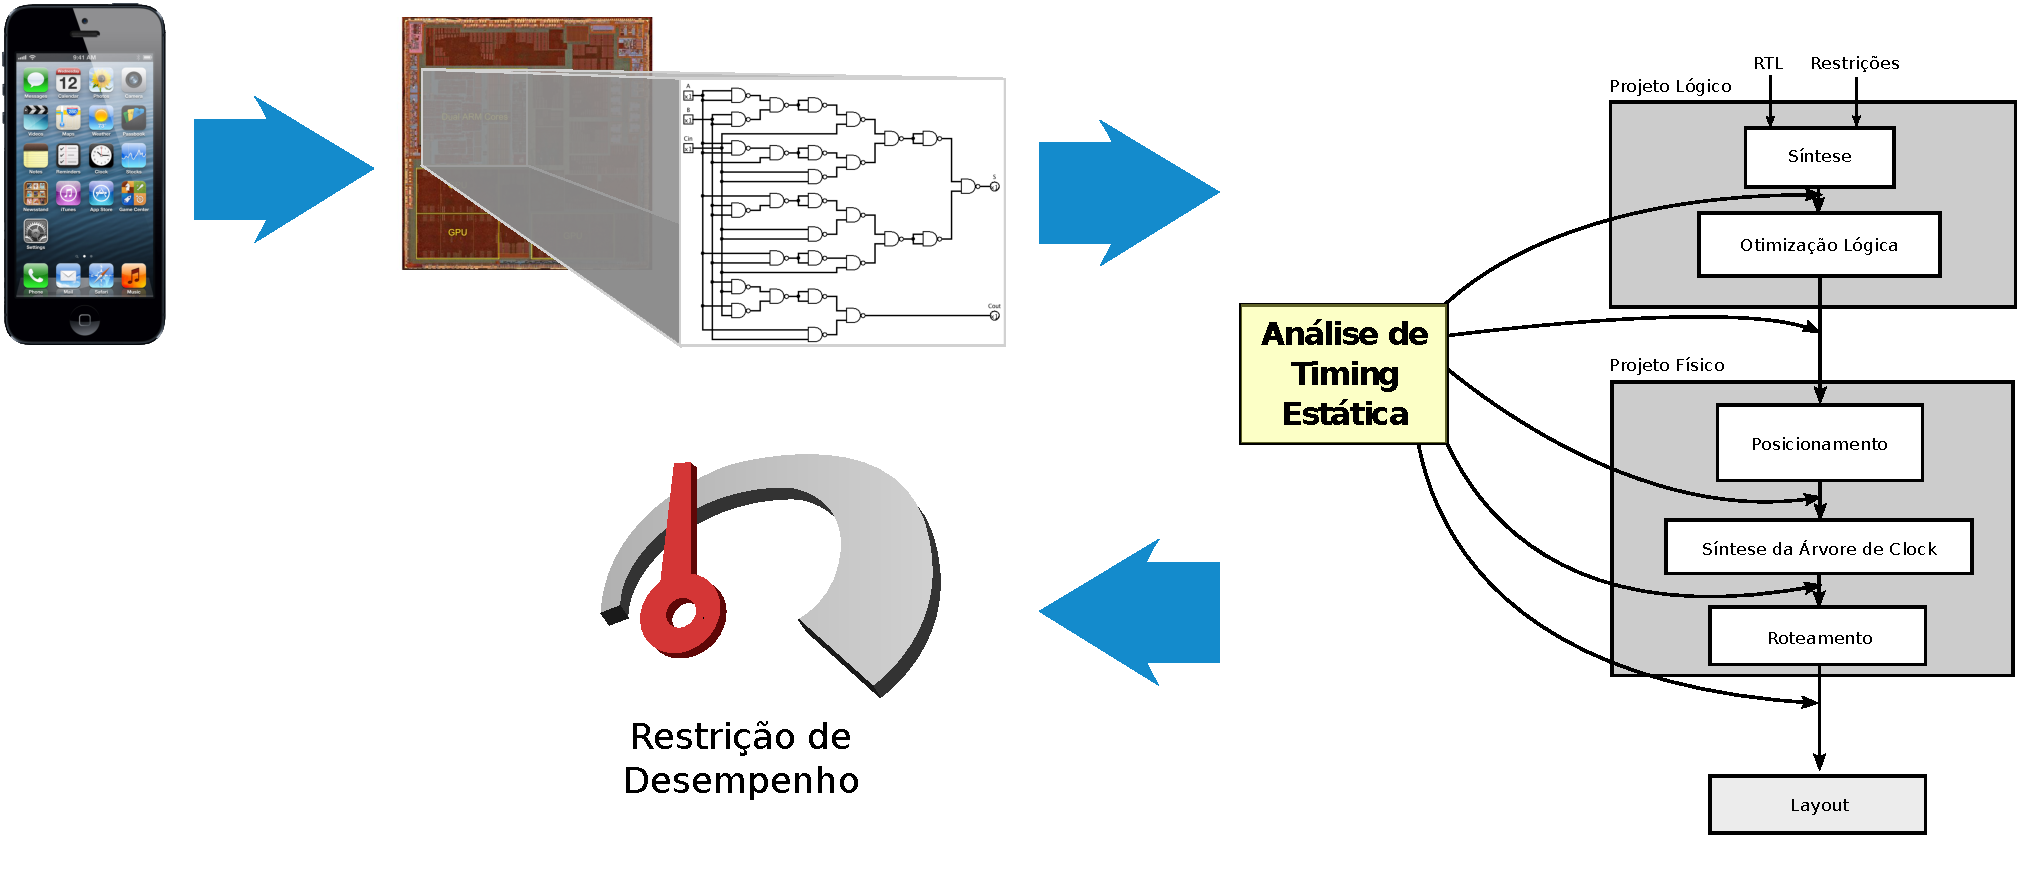
\includegraphics[width=1.05 \linewidth, trim=2cm 0 0 0]{img/motivacao.pdf} 
%				\end{center}
%					
%				\begin{itemize}
%					\item Necessidade de um \textit{time-to-market} curto;
%					\item Adoção do fluxo \textit{standard cell}.
%				\end{itemize}
%			\end{frame}
			\begin{frame}
				\frametitle{Motivação}
				\pgfdeclareimage[width=1.1 \linewidth]{motivacao1}{img/motivacao1.pdf}
				\pgfdeclareimage[width=1.1 \linewidth]{motivacao2}{img/motivacao2.pdf}
				\pgfdeclareimage[width=1.1 \linewidth]{motivacao3}{img/motivacao3.pdf}
				\pgfdeclareimage[width=1.1 \linewidth]{motivacao4}{img/motivacao4.pdf}
				\pgfdeclareimage[width=1.1 \linewidth]{motivacao5}{img/motivacao5.pdf}


				\pgfuseimage{motivacao1}<1>
				\pgfuseimage{motivacao2}<2>
				\pgfuseimage{motivacao3}<3>
				\pgfuseimage{motivacao4}<4>
				\pgfuseimage{motivacao5}<5>
				
			
			\end{frame}
			
		
			\begin{frame}
				\frametitle{Motivação: Fluxo \textit{Standard Cell}}
				\begin{minipage}{0.5 \textwidth}
					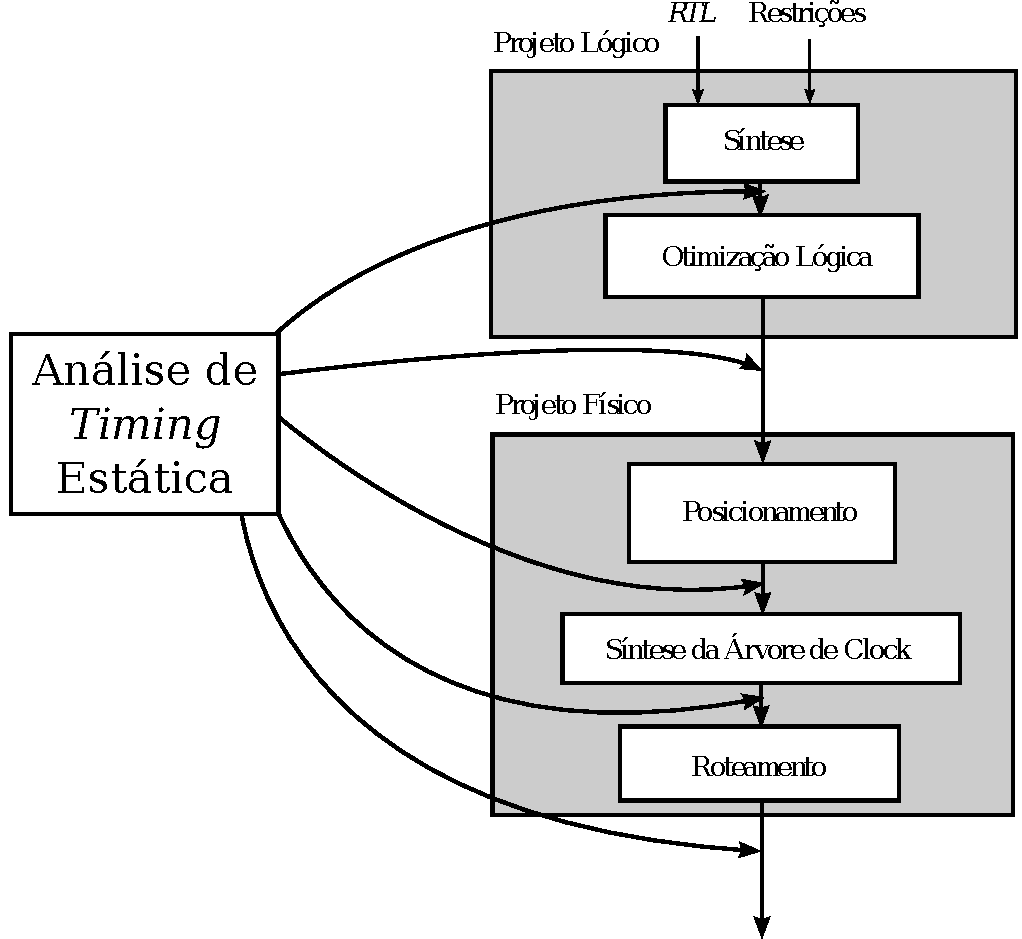
\includegraphics[width=\textwidth]{img/fluxo_standard_cell.pdf}
				\end{minipage}
				\begin{minipage}{0.4 \textwidth}
					\begin{itemize}
						\item Diversas otimizações:
							\begin{itemize}
								\item Área;
								\item Potência;
								\item Atraso Máximo.
								
							\end{itemize}
						\item Avaliação das informações temporais nas mais diversas etapas do fluxo.
					\end{itemize}
				\end{minipage}
				
			\end{frame}
		
			\begin{frame}
				\frametitle{Justificativa}
				\begin{itemize}
					\item Inexistência de ferramentas de STA em domínio público;
					\item Alto custo das licenças das ferramentas industriais.
				\end{itemize}
			\end{frame}
		
			\begin{frame}
				\frametitle{Objetivos}
				\begin{itemize}
					\item Projeto, avaliação, validação e documentação de uma ferramenta de STA voltada para o fluxo \textit{standard cell.}
					\begin{enumerate}
						\item Modelo de interconexão de capacitância concentrada; \label{obj:1}
						\item Técnica de Elmore para cálculo dos atrasos das interconexões; \label{obj:2}
						\item Técnica para o cálculo do atraso das interconexões utilizando a abordagem de capacitância efetiva; \label{obj:3}
						\item Construção de uma ferramenta de STA que implementa \ref{obj:1}, \ref{obj:2} e \ref{obj:3}. 
					\end{enumerate}
				\end{itemize}
			\end{frame}
			
			\begin{frame}
				\frametitle{Escopo}
				\begin{itemize}
					\item Modelos de atraso adotados em fluxo \textit{standard cell};
					\item 2 modelos de interconexão:
						\begin{enumerate}
							\item Modelo de Capacitância Concentrada
							\item Modelo RC Concentrado
						\end{enumerate}
					\item \textbf{NÃO} faz parte do escopo:
					\begin{itemize}
						\item Tempos de \textit{setup} e \textit{hold} das células sequenciais;
					\end{itemize}
				\end{itemize}
				
				
			\end{frame}
		
	
	\section{Conceitos}
		
		\begin{frame}
		\frametitle{Características Temporais dos Circuitos Digitais}
			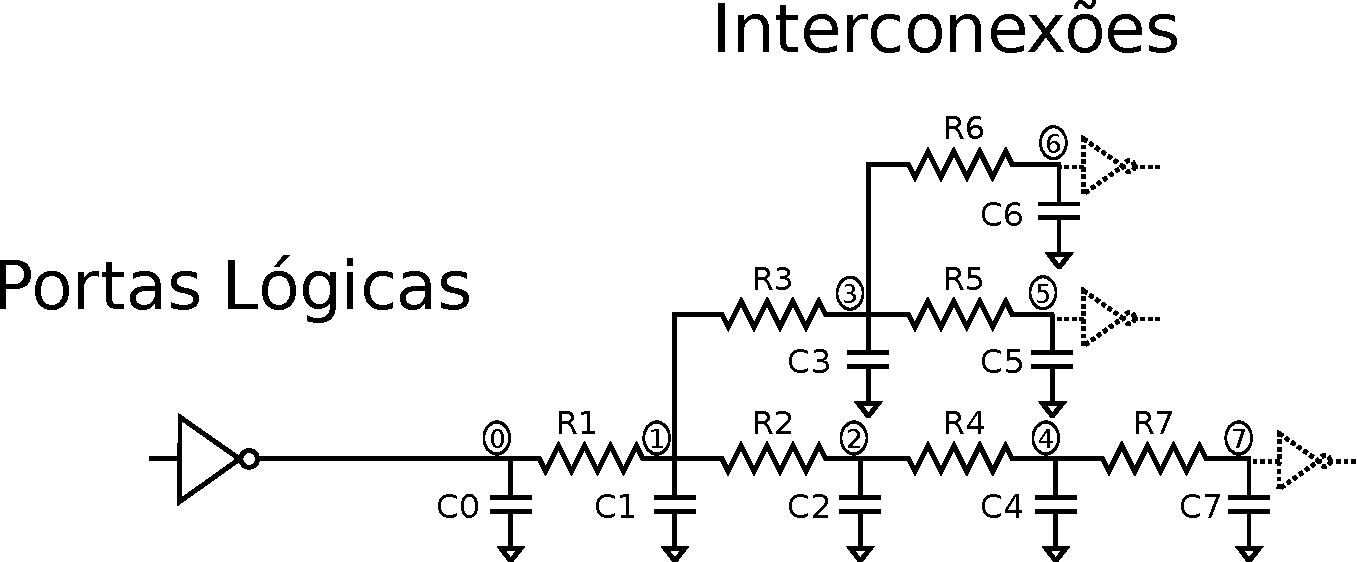
\includegraphics[width=\textwidth]{img/circuito.pdf} 
		\end{frame}

		\subsection*{Portas Lógicas}
			\begin{frame}
				\begin{center}
					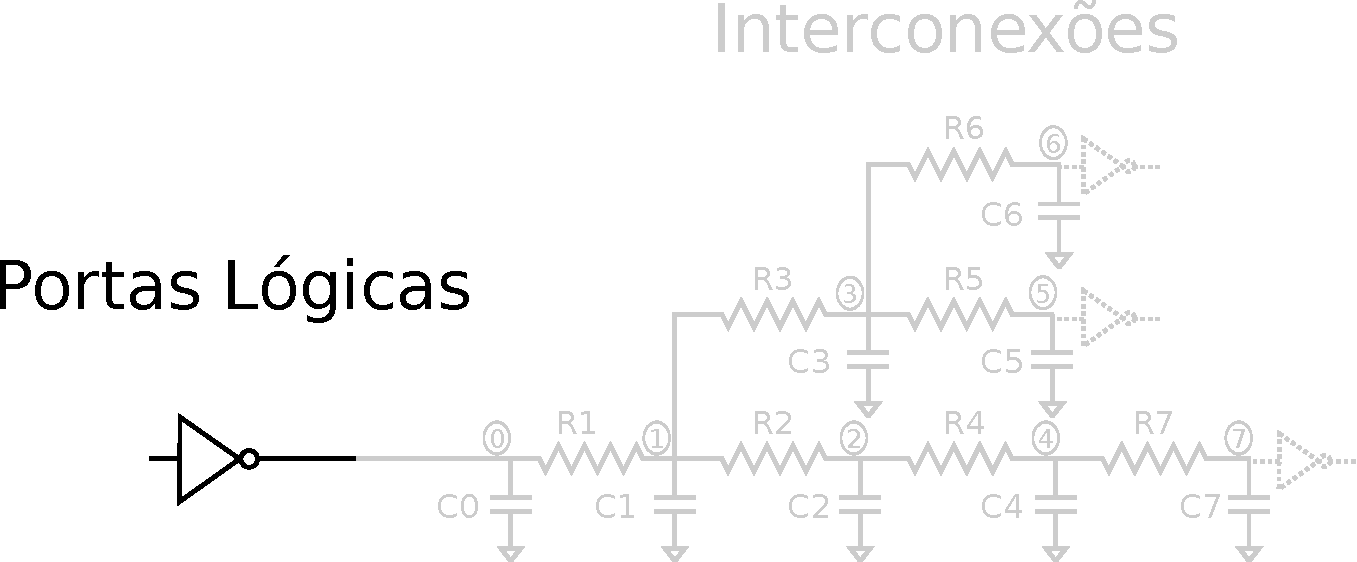
\includegraphics[width=\textwidth]{img/circuito_portas.pdf} 
				\end{center}
			\end{frame}
			
			\begin{frame}
				\frametitle{Características Temporais}
				\begin{itemize}
					\item \textit{Timing Arc} e \textit{Driver} \\		
						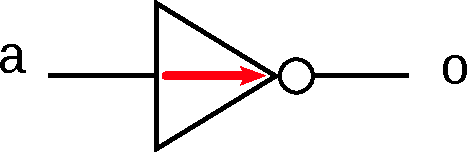
\includegraphics[width=0.3 \textwidth]{img/carac_portas_1.pdf}
					\item \textit{Delay} \\ 
						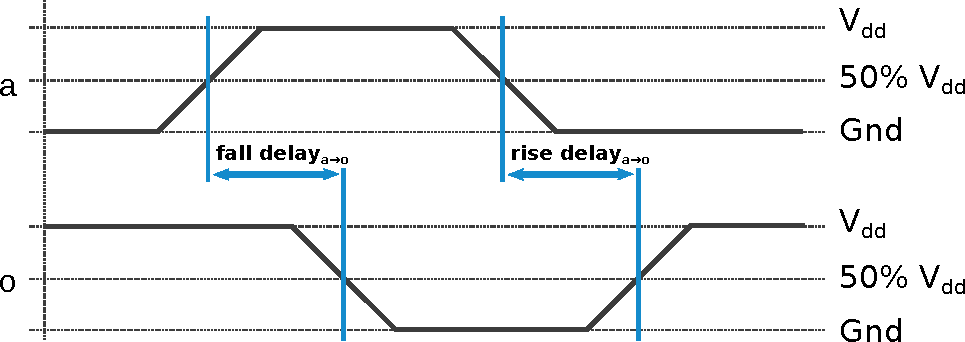
\includegraphics[width=0.7 \textwidth]{img/carac_portas_2.pdf}
					\item \textit{Slew} \\
						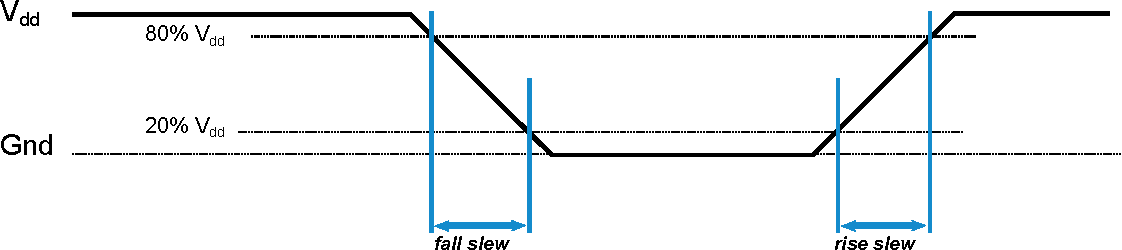
\includegraphics[width=0.7 \textwidth]{img/carac_portas_3.pdf}  
				\end{itemize}

				
			\end{frame}
			
			\begin{frame}
				\frametitle{Modelo de Atraso Não-Linear}
					\begin{center}
						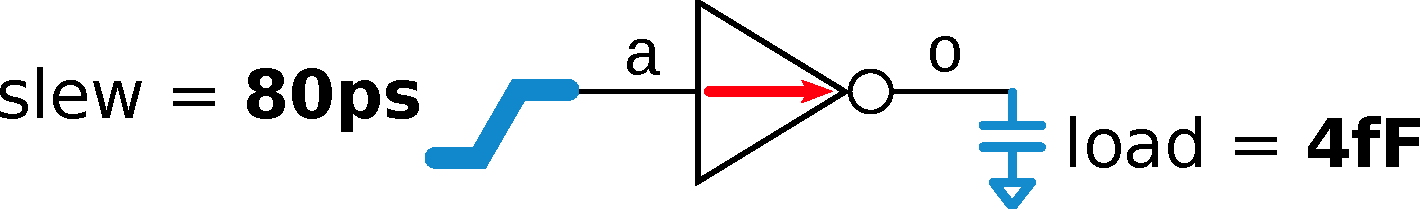
\includegraphics[width=0.7\textwidth]{img/nldm_1.pdf}
					\end{center}
					
					\begin{itemize}
						\item \textit{Delay}: $f(slew, load) = 52.05ps $	\\
						\begin{center}
							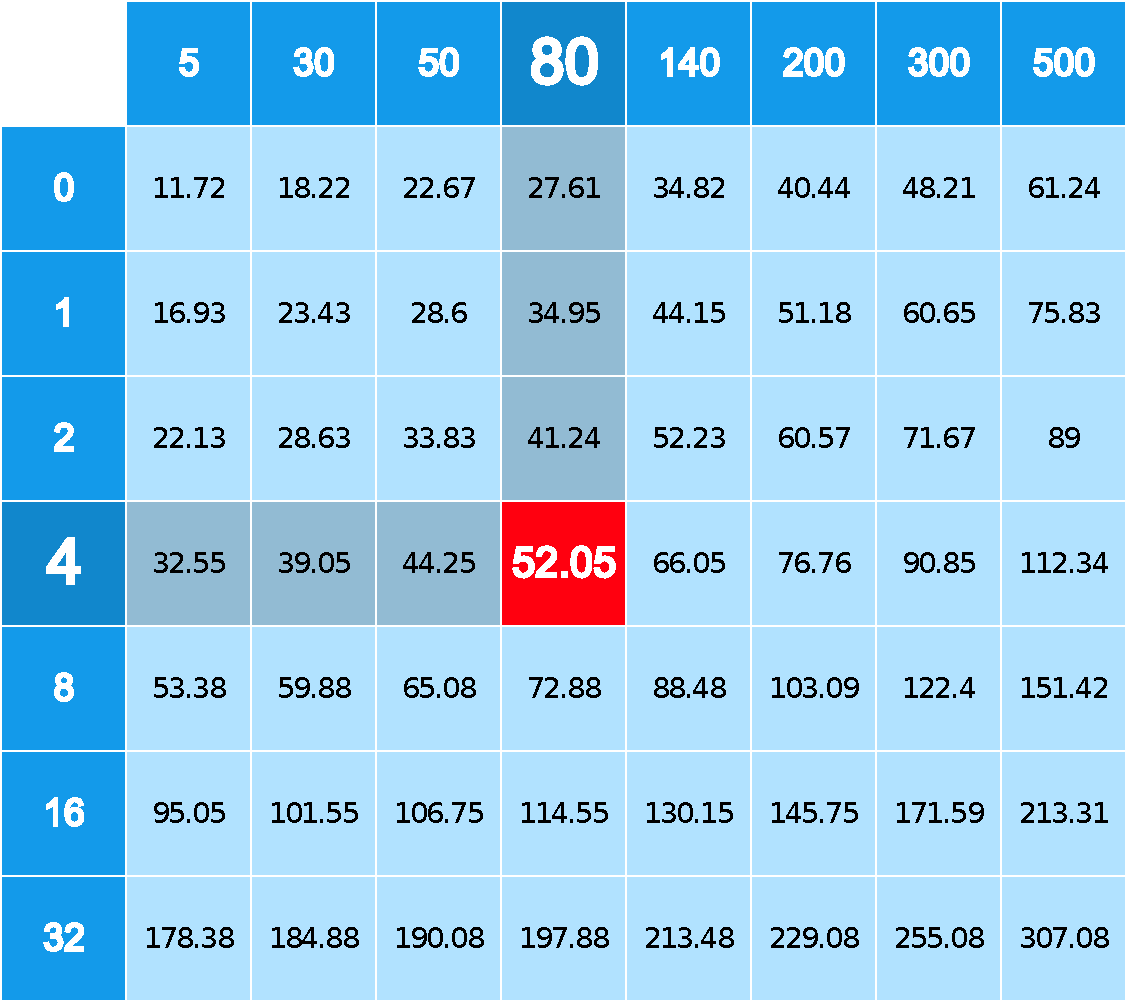
\includegraphics[width=0.4 \linewidth]{img/nldm_2.pdf} 
						\end{center}
					\end{itemize}					
						
			\end{frame}
		
		\subsection*{Interconexões}

			
			\begin{frame}
				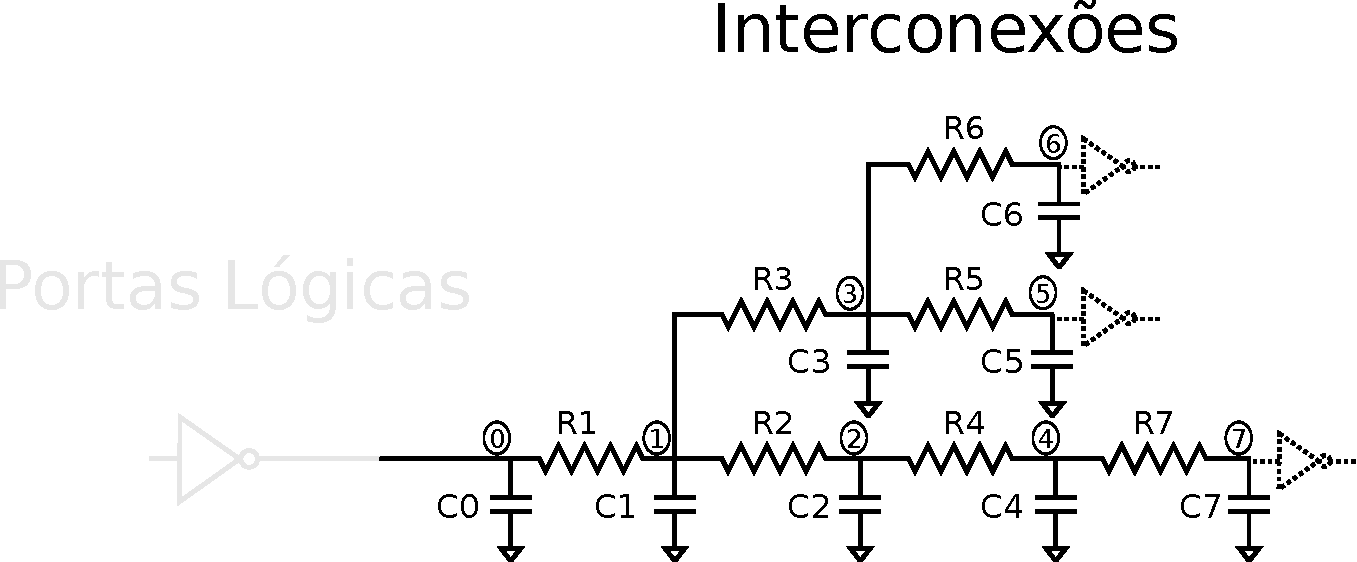
\includegraphics[width=\textwidth]{img/circuito_interconexao.pdf} 
			\end{frame}
			
			\subsubsection*{Modelos de Interconexões}
				\begin{frame}
					\frametitle{Modelo RC Distribuído}
					\begin{center}
						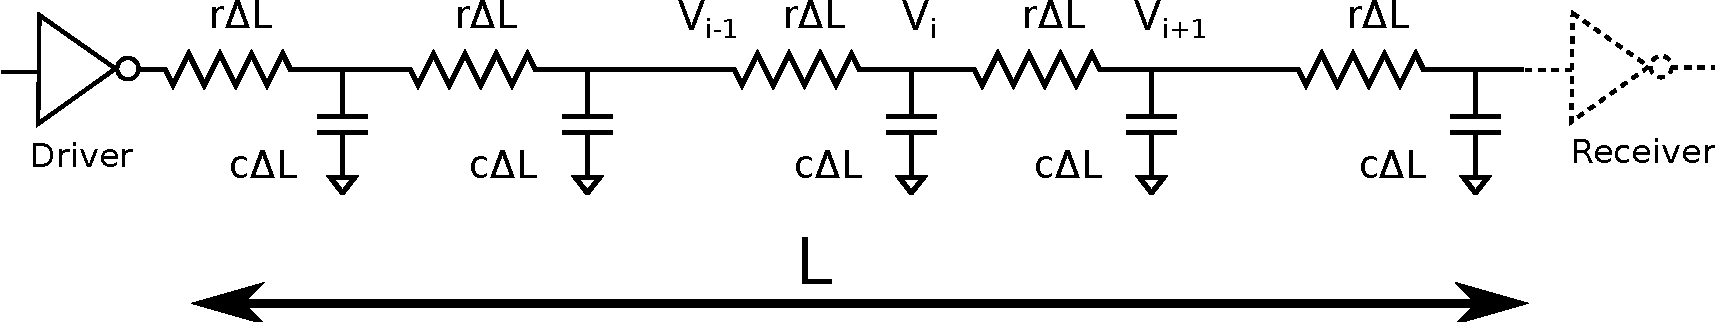
\includegraphics[width=\textwidth]{img/distributed_rc.pdf} 
					\end{center}
					\begin{itemize}
						\item Cálculo do atraso reflete na solução de equações diferenciais;
						\item Não possui fórmula fechada;
						\item Modelos de interconexão simplificados são mais adotados em fluxo \textit{standard cell}.
					\end{itemize}
					
					
				\end{frame}
				
				\begin{frame}
					\frametitle{Modelo de Capacitância Concetrada}
					\begin{center}
						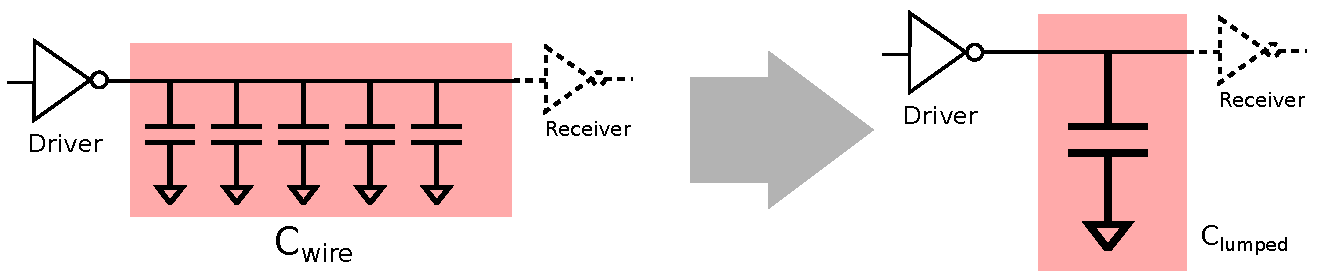
\includegraphics[width=\textwidth]{img/lumped_c.pdf} 
					\end{center}
					\begin{itemize}
						\item Modelo utilizado quando a resistência da interconexão é despresível;
						\item Concentra-se toda a capacitância da interconexão em um único capacitor;
						\item Seu atraso é desconsiderado.
					\end{itemize}							
				\end{frame}
				
				\begin{frame}
					\frametitle{Modelo de RC Concentrado}
					\begin{center}
						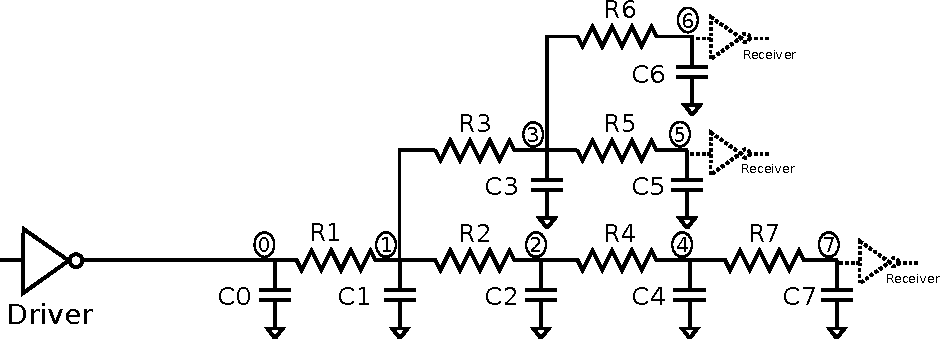
\includegraphics[width=\textwidth]{img/lumped_rc.pdf} 
					\end{center}
					\begin{itemize}
						\item Modelo amplamente adotado em fluxo \textit{standard cell};
						\item Concentra-se toda a resistência de cada segmento  em um único resistor R;
						\item Combina-se a capacitância total em um único capacitor C;
						\item Árvore RC.
					\end{itemize}								
				\end{frame}
			
			\subsubsection*{Características Temporais}
			\begin{frame}
				\frametitle{Características Temporais}
				
				
					\begin{figure}
						\subfigure[]
						{
						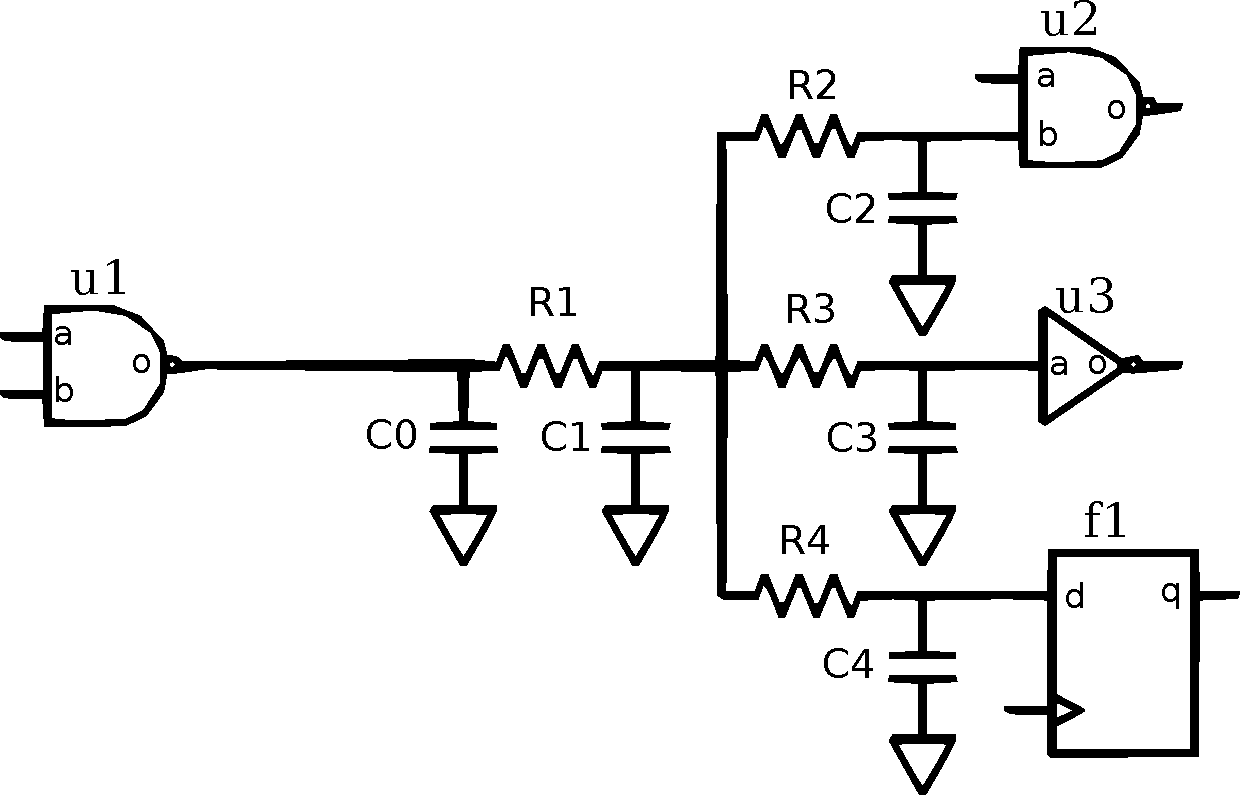
\includegraphics[width=0.4 \textwidth]{img/modelagem1.pdf}
						}
						\subfigure[]
						{
						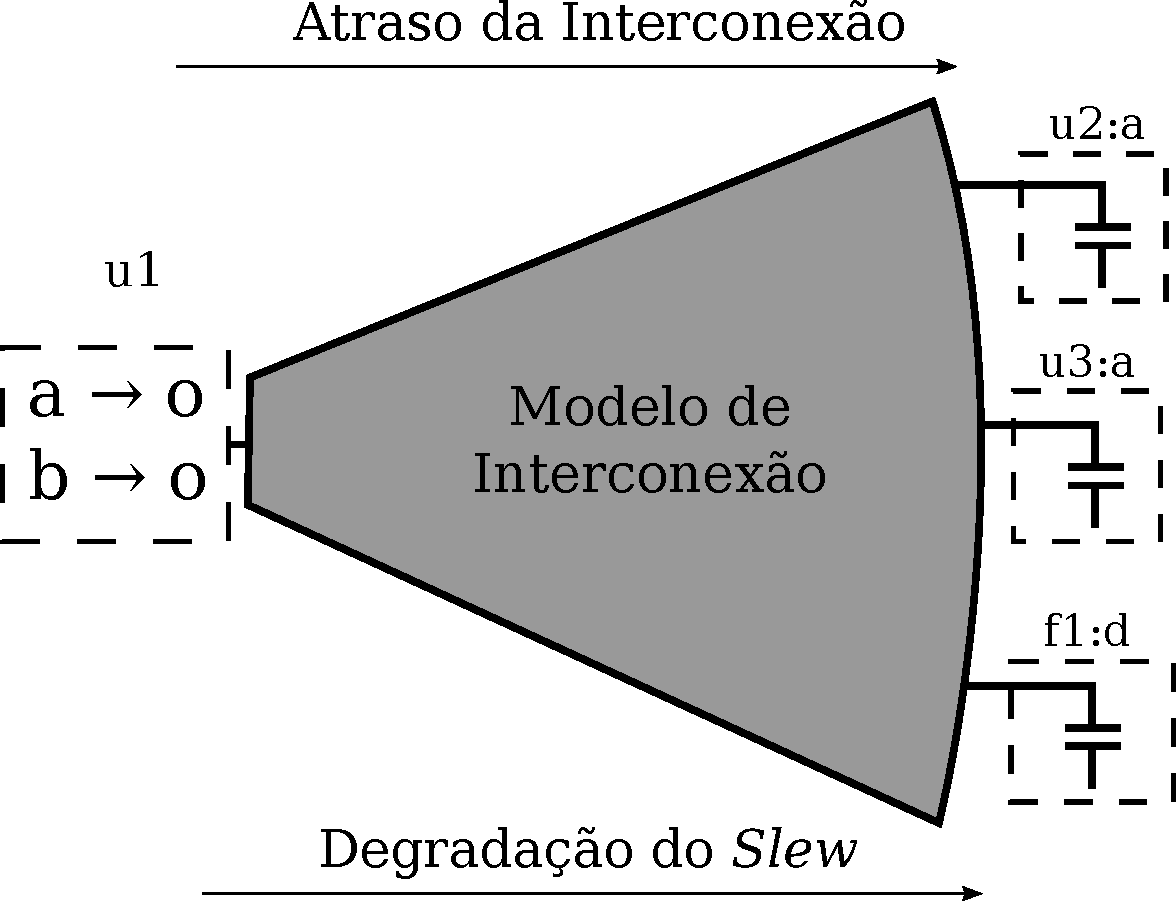
\includegraphics[width=0.4 \textwidth]{img/modelagem2.pdf}
						}
						
					\end{figure}
					
					\begin{itemize}
						\item Capacitância ``Vista'' Pelo \textit{Driver};
						\item Atraso da Interconexão;
						\item Degradação do \textit{Slew}. 		
					\end{itemize}
			\end{frame}
	
	\section{Trabalhos Correlatos}
	
		\begin{frame}
		\frametitle{Trabalhos Correlatos}
			\begin{itemize}
				\item<1> AWE
				\item<1> PRIMA
				\item<1> Kashiyap
				\item<1> Puri
			\end{itemize}
		\end{frame}
	
	\section{Técnica Implementada}
	
		\begin{frame}
			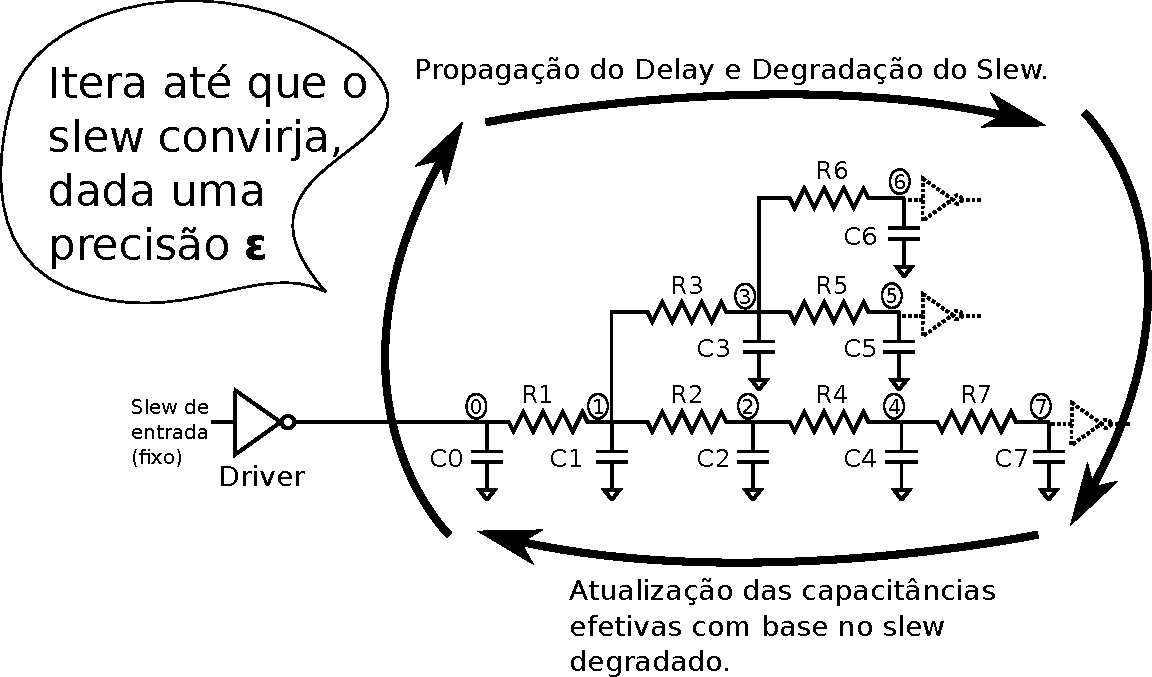
\includegraphics[width=\textwidth]{img/imagem_puri.pdf} 
		\end{frame}
		
		\begin{frame}
			\begin{minipage}{0.4\textwidth}
				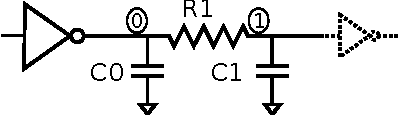
\includegraphics[width=\textwidth]{img/pi.pdf} 

			\end{minipage}
			\begin{minipage}{0.5\textwidth}
				\begin{itemize}
					\item<1-3> \textbf{Capacitância efetiva:}\\
						$C_{eff_0} = C_0 + C_1 \times K$ 
						$K = 1 - 2x(1 - e^{-\frac{1}{2x}})$
						$x = \frac{R_1C_1}{slew_1}$
					\item<2-3> \textbf{Atraso da interconexão:} \\
						$\tau_1 = \tau_0 + R_1 \times C_1$
					\item<3> \textbf{Degradação do \textit{slew}: }
						$slew_1 = \frac{slew_0}{1 - \frac{R_1 C_1}{slew_0} (1 - e^{-\frac{slew_0}{R_1 C_1}})}$
				\end{itemize}
			\end{minipage}
		\end{frame}
	
	\section{Análise de Timing Estática}
	
		\begin{frame}
		sta sta
		\end{frame}
	
	\section{Experimentos}
	
		\begin{frame}
		experimentos
		\end{frame}
	
	\section{Conclusões}
	
		\begin{frame}
		conclus~oes
		\end{frame}
	
	\section{Trabalhos Futuros}
		
		\begin{frame}
		trabalhos
		\end{frame}
	
\end{document}
